\subsection{Dilation}
Figur~\ref{fig:dilation1} og \ref{fig:dilation2} viser dilation. 

Bruges eksempelvis til at udfylde huller. Lukke 'gaps' etc.

\begin{figure}[H]
	\centering
	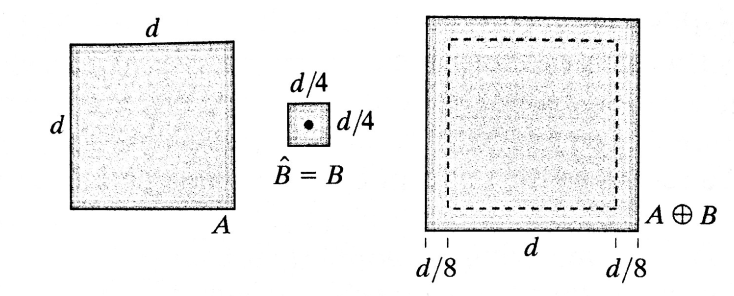
\includegraphics[width=0.7\linewidth]{figs/spm09/dilation1}
	\caption{Eksempel på dilation med 4x4 strel.}
	\label{fig:dilation1}
\end{figure}

\begin{figure}[H]
	\centering
	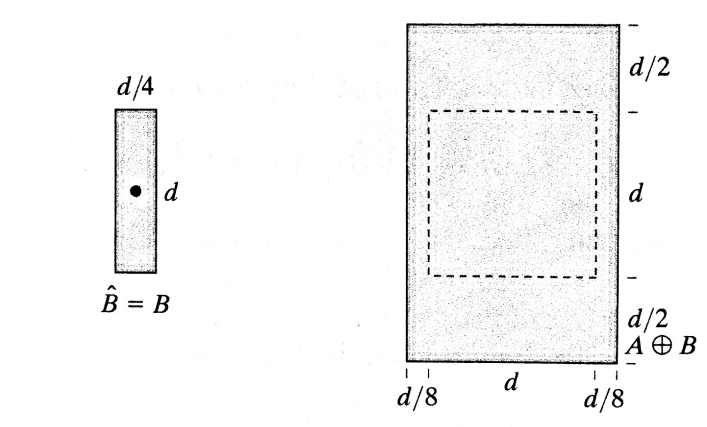
\includegraphics[width=0.7\linewidth]{figs/spm09/dilation2}
	\caption{Eksempel på dilation med aflangt strel.}
	\label{fig:dilation2}
\end{figure}

De matematiske udtryk for dilation ses på Figur~\ref{fig:dilationeq1}.

\begin{figure}[H]
	\centering
	
\includegraphics[width=0.6\linewidth]{figs/spm09/dilationeq1}
	\caption{Ligning for dilation.}
	\label{fig:dilationeq1}
\end{figure}
